%this file is the second report
%a % comment anything after % until the end of the line

%minimum references to begin our article
\documentclass[12pt]{article}
\usepackage[english]{babel}
\usepackage[utf8]{inputenc}
\usepackage[T1]{fontenc}
\usepackage{graphicx}
\usepackage{fancyhdr}
\usepackage{hyperref}
\usepackage{float}
\usepackage{enumitem}
\usepackage{amsmath}
\usepackage[margin=1in]{geometry}
\usepackage{indentfirst}
\usepackage{titlesec}
\usepackage{url}
\newcommand{\sectionbreak}{\clearpage}

%\setlength{\parskip}{10pt plus 1pt minus 1pt} %Adds spacing between paragraphs 
\usepackage{parskip}
\setlength{\parindent}{15pt}

\pagestyle{fancy}
%\cfoot{Fast and furious game playing: Monte Carlo drift}
% the last extension makes it possible to add images

%presentation of the document
\title{Fast and Furious Game Playing: Monte Carlo Drift\smallbreak Specifications report} %not sure about the name of this report
\author{Prateek \textsc{Bhatnagar}, Baptiste \textsc{Bignon}, \\
        Mikaïl \textsc{Demirdelen}, Gabriel \textsc{Prevosto}, \\
        Dan \textsc{Seeruttun-{}-Marie}, Benoît \textsc{Viguier} \\
        \\
        Supervisors: Nikolaos \textsc{Parlavantzas}, Christian \textsc{Raymond}}
\date{11/27/2014}
\setlength\parindent{15pt}
\begin{document}
\maketitle

\begin{figure}[!h] 
\centerline{\includegraphics[scale=0.50]{Pictures/arimaa}}
\end{figure}
\newpage


\begin{abstract}
%put abstract here
	This second report is related to the incremental development of the project \textit{Fast and Furious Game Playing: Monte Carlo Drift}. This report is about the specifications of the project.
A detailed study has been reported here about various components of the project. This report is a step ahead of the previous report and focuses on "what" factor ,about each and every component of the project that includes  game, general architecture, application programming interface, Artificial Intelligence- implementation of  MCTS Algorithm, User Interface and Application Program. A detailed focus is also made on the parallelisation techniques using OpenAcc and OpenMP.
\end{abstract}
\newpage

%to add a table of contents
\tableofcontents
\newpage


\section{Introduction}						\label{sec:introduction} 		
In 1997, Deep Blue, a supercomputer built by IBM, won a six games match against Garry Kasparov, the current world chess champion. Humans got beaten in Chess, but remain undefeated in other games. Consequently, researchers are looking for improvements in Artificial Intelligence.
\newline

The project is called \emph{Fast \& Furious Game Playing, Monte Carlo Drift}. Its purpose is to create an Artificial Intelligence able to compete against humans using the \emph{Monte Carlo Tree Search}.
\newline

The focus of this project is on two player strategy board games, while avoiding games already solved\footnote{A game solved is a game where good algorithms are able to find the perfect move in each situation to win, or to draw. For instance, \textit{Tic Tac Toe} or \textit{Draughts} are solved games.}. That is why this project is about the game \emph{Arimaa}.
\newline

A human plays a game by thinking of all possible moves as per one's imagination and then opts the best amongst them. The player can be able to look further for the opponent's turn, and it expands possibilities of moves. The Minimax algorithm does exactly the same thing, but it is exploring all possibilities. The current position is represented by a node, and the possible states after a move are represented by other nodes, pointing to the parent node. Then it forms a tree.
Minimax algorithm develops a tree by creating nodes for all possible moves.
\newline

The problem is to compute this heavy algorithm. The \emph{MCTS} algorithm has been conceived to choose to develop some of the nodes, so it will be use for our project.
The \emph{Monte Carlo Tree Search} has been used in the past for \textit{Draughts}. By exploring numerous random possibilities, it will be able to take decisions in order to win a game of \emph{Arimaa}.
The algorithm would be parallelized in order to exploit it in a multi-core machine, allowing it to go further into the search tree, thus improving its efficiency.
\newline

Different parallelization methods will be studied in order to choose the most suitable, for this project.
The exploration of the tree will depend on the parallelization method.
The initial phase of the project would be the analysis of the latest papers concerning the technologies that might be of use.
The consecutive phases will be about making a choice among these technologies, to decide on the specifications.
Finally, in the last phase, a solution will be implemented, and executed on Grid'5000, a cluster of multi-core machines.
\newline

In this report, the first part will be about the presentation of Arimaa (see part \ref{first part}.) Then, different algorithms about the game will be introduced (see part \ref{second part}). The third part will be consacred to parallelization methods (see part \ref{third part}) and the state of the art (see part \ref{third part part}). In the end, solutions (see part \ref{last part}) and the schedule will be presented (see part \ref{last last part}).
The interesting part about this project is the creation of an artificial intelligence as optimized as possible.
\newpage

\section{Algorithmic methods}
An explanation of our methods and concepts is necessary to understand how our project works. The use of some parallelization methods, and the MCTS algorithm is here developed.					\label{sec:algorithmicMethods}
	\subsection{Parallelization methods}			\label{sec:parallelization}		In order to increase the speed of our program, we have decided to parallelize it on a set of clusters of multi-core machines. But there are many ways to parallelize our algorithm and we have to choose how we want to do it. 
\subsubsection{Previous Work}
In the last report, we talked about the different methods, their advantages and their drawbacks. We have seen that there are mainly two parallelization methods that are efficient in our project.

The first one is called the Root Parallelization. It consists in giving the tree to develop to every thread, let them develop it randomly without any communication with the environment
during a certain amount of time and then, merge the results of each tree.
This method has the great benefit of minimizing the communication between the actors (in this case, the threads).
They only communicate at the beginning and at the end of the algorithm, without needing any further synchronization. The Root Parallelization is depicted in figure \ref{fig:root}.

\begin{figure}[!h] 
\centerline{\includegraphics[scale=0.60]{3Methods/3.1Parallelization_Method/root.png}}
   \caption{Overview of Root Parallelization}
\label{fig:root}
\end{figure}

The other efficient parallelization method is called UCT-Treesplit and is depicted if figure \ref{fig:treesplit}. It looks like Root Parallelization as we give to each actor the same tree to develop.
But contrary to Root Parallelization, when the tree is developed on a certain node, it goes on working packages who are distributed among every actor. %Me not understand sentence
In terms of performance, this method is very efficient but needs an High-Performance Computer, or \emph{HPC}, and is very sensitive to network latency.

\begin{figure}[!h] 
\centerline{\includegraphics[scale=0.80]{3Methods/3.1Parallelization_Method/treesplit.png}}
   \caption{Overview of UCT-Treesplit Algorithm}
\label{fig:treesplit}
\end{figure}


We have to choose two parallelization methods, one for the cluster parallelization and another for the shared memory parallelization.
\subsubsection{Cluster Parallelization}
For the cluster parallelization, we have to take into account the fact that we will need to communicate by sending messages, that are relatively costly in terms of performance.
Moreover, as the network can have latency, we should minimize the communication between the computers and that's why we have choose to implement a Root Parallelization.
It reduces the cost in communication at maximum, is very simple to implement, does not depend on the configuration of each computer and is very efficient.
\subsubsection{Shared Memory Parallelization}
For the shared memory parallelization we could choose both Root Parallelization or UCT-Treesplit.
If we choose UCT-Treesplit, it may be difficult to implement it correctly since it is a very complex strategy and, moreover, it would make the algorithm very sensitive to network issues. That is why we chose to implement another Root Parallelization. This way, the global strategy of our program will be simple and homogeneous.

	\subsection{Monte Carlo Tree Search algorithm}		\label{sec:mcts}			%this file is the second report
%a % comment anything after % until the end of the line

%minimum references to begin our article
\documentclass[12pt]{article}
\usepackage[english]{babel}
\usepackage[utf8]{inputenc}
\usepackage[T1]{fontenc}
\usepackage{graphicx}
\usepackage{fancyhdr}
\usepackage{hyperref}
\usepackage{float}
\usepackage{amsmath}
\usepackage[margin=1in]{geometry}
\usepackage{indentfirst}
\usepackage{titlesec}
\newcommand{\sectionbreak}{\clearpage}

\pagestyle{fancy}
%\cfoot{Fast and furious game playing: Monte Carlo drift}
% the last extension makes it possible to add images

%presentation of the document
\title{Fast and Furious Game Playing : Monte Carlo Drift\smallbreak Specifications report} %not sure about the name of this report
\author{Prateek \textsc{Bhatnagar}, Baptiste \textsc{Bignon}, \\
		Mikaïl \textsc{Demirdelen}, Gabriel \textsc{Prevosto}, \\
		Dan \textsc{Seeruttun-{}-Marie}, Benoît \textsc{Viguier} \\
		\\
		Supervisors: Nikolaos \textsc{Parlavantzas}, Christian \textsc{Raymond}}
\date{11/27/2014}
\setlength\parindent{15pt}
\begin{document}
\maketitle

The MCTS algorithm has been chosen in order to develop our artificial intelligence. However, in order to improve its efficiency, we will need to tweak it a bit. The main problem is the branching factor\footnote{In a tree,  the branching factor is the number of children at each node.} of the Arimaa game which average is 17 281 and reaches about 22 000 after 10 moves.
\bigskip
\begin{center}
	\begin{tabular}{ | c | c |}
		\hline Game & Average number of possible moves \\ \hline
		\hline  
		Othello & 8\\
		\hline  
		Chess & 35\\
		\hline  
		Game of Go & 250\\
		\hline
		Arimaa & 17 281\\
		\hline
	\end{tabular}
\end{center}
\bigskip
The reason why the branching factor of a game is so important is because it increases greatly the space that has to be searched in order to guess what will happend multiples moves ahead. In chess after 6 moves, the number of positions evaluated are about 35\textsuperscript{6} which is roughtly equivalent to 1,8 billions. In Arimaa, after 3 turns (yours, the opponent and yours again), if you were the explore all positions, you would need to evaluate around 5,2 trillions\footnote{1 trillion = 1 thousand billions = 10\textsuperscript{12}.} boards (2000 times more than chess with half the number of moves).

\end{document}

\newpage

\section{General Architecture}					\label{sec:generalArchitecture} 		
	\subsection{Introduction}			\label{sec:gameBehavioiur}		An application will be developed in order to test the AI\footnote{Artificial Intelligence} against human players as well as other AIs.
In our project, the AI is handled by the MCTS algorithm. We'll see more on its implementation on part \ref{sec:mctss}.
Our application will integrate four modules: 
\begin{itemize}
\item the Artificial Intelligence
\item the game model containing the rules
\item the user interface (\emph{UI}) described in part \ref{sec:ui}
\item an \emph{API} described in part \ref{sec:api} that will be used to integrate other AIs
\end{itemize}

In this part, the different interactions between these modules will be discussed.
The UI, as well as the algorithm for the AI, will act upon the game model, so as to inform it of what moves were made.
The UI will also regularly update to give the player feedback on the progression of the game (for more details, see part \ref{sec:globalview}).

If at some point our AI is to be tested against an AI created by others, an API will be needed in order to interface it with the game model, as described in part \ref{sec:api}.

	\subsection{Context of the architecture}		\label{sec:globalview}			The organization of the architecture is described in Figure \ref{fig:gen}.

\begin{figure}[!h]
\centering
\includegraphics[width=0.5\textwidth]{2General_Architecture/2.1.2GeneralView/gen.png}
\caption{General view of the architecture}
\label{fig:gen}
\end{figure}

The user will interact with the user interface, which will communicate with the game application, where all data for the game will be stored. Then, it will communicate with an Interface which will handle the communications between the Game application and the computer player. 

In our case, the computer player will be played by the AI using the MCTS algorithm, communicating with the Arimaa set of rules via the API and an interface for the set of Rules.  If another algorithm is to be tested, it will be added.

Interfaces are very important because they make it possible for others to use our project for others games than Arimaa without rebuilding everything. They would only have to implement the Interface with their proper game, game rules.

Furthermore, if the time permits it, the management of computers bots\footnote{For instance of the site \textit{Arimaa.com}} will be added. The only problem here is the computers bots are not similar to each other, thus it will take time to implement a class which will be able to communicate with both the computer bot and the interface.

The input of our software will be provided by the user using the mouse and keyboard. The output will only be the display of the screen, after the computer player makes a move.
	\subsection{User Interface module}				\label{sec:ui}				In order to test our program against human players, we will develop an application implementing a graphical user interface (\emph{GUI} or also \emph{UI}).
This application will interface directly with the model.
It will be controllable by the human with the mouse or keyboard, in a manner as intuitive as possible.
Thanks to this UI, the user will be able to choose between a one-player mode, a two-plaer mode and a demonstration mode.
This last mode consists in a match between two AIs, and will be helpful to compare different AIs.
The user will also be able to choose the parameters for the AIs, if we have time to develop more than one.
	\subsection{Converter module}		\label{sec:api}				<<<<<<< HEAD
API stands for Application Programming Interface. API, is a set of routines, protocols, and tools for building software applications. The API specifies how software components should interact and are used when programming graphical User Interface (GUI) components. A good API makes it easier to develop a program by providing all the building blocks. A programmer then puts the blocks together.\bigbreak
 In this project the API will be induced between the MCTS algorithm i.e. AI and the board game application and will be responsible for providing the input to the board game application in understandable format and will receive the input from the MCTS algorithm. The following diagram will help in understanding the things better.
=======
API stands for Application Programming Interface. An API is a set of routines, protocols, and tools for building software applications. The API specifies how software components should interact and are used when programming graphical User Interface (GUI) components. A good API makes it easier to develop a program by providing all the building blocks. A programmer then puts the blocks together.

 In this project the API will be induced between the MCTS algorithm and the board game application. It will be responsible for providing the input to the board game application in understandable format and will receive the input from the MCTS algorithm. Its usage is described in figure \ref{fig:flowchart}.
>>>>>>> 7a721ccb0b918408612e06d9354ae24b531db0a1

\bigbreak

\begin{figure}[H]
	\centering
	\includegraphics[width=\textwidth]{2General_Architecture/2.2API/img/DiagramAPI.png}
	\caption{The flowchart describing the usage of the API}
	\label{fig:flowchart}
\end{figure}



	\subsection{The MCTS Algorithm module}		\label{sec:mctss}				The next Figure \ref{fig:flow} describes the AI, i.e. the MCTS Algorithm module.

\begin{figure}[H]
	\centering
	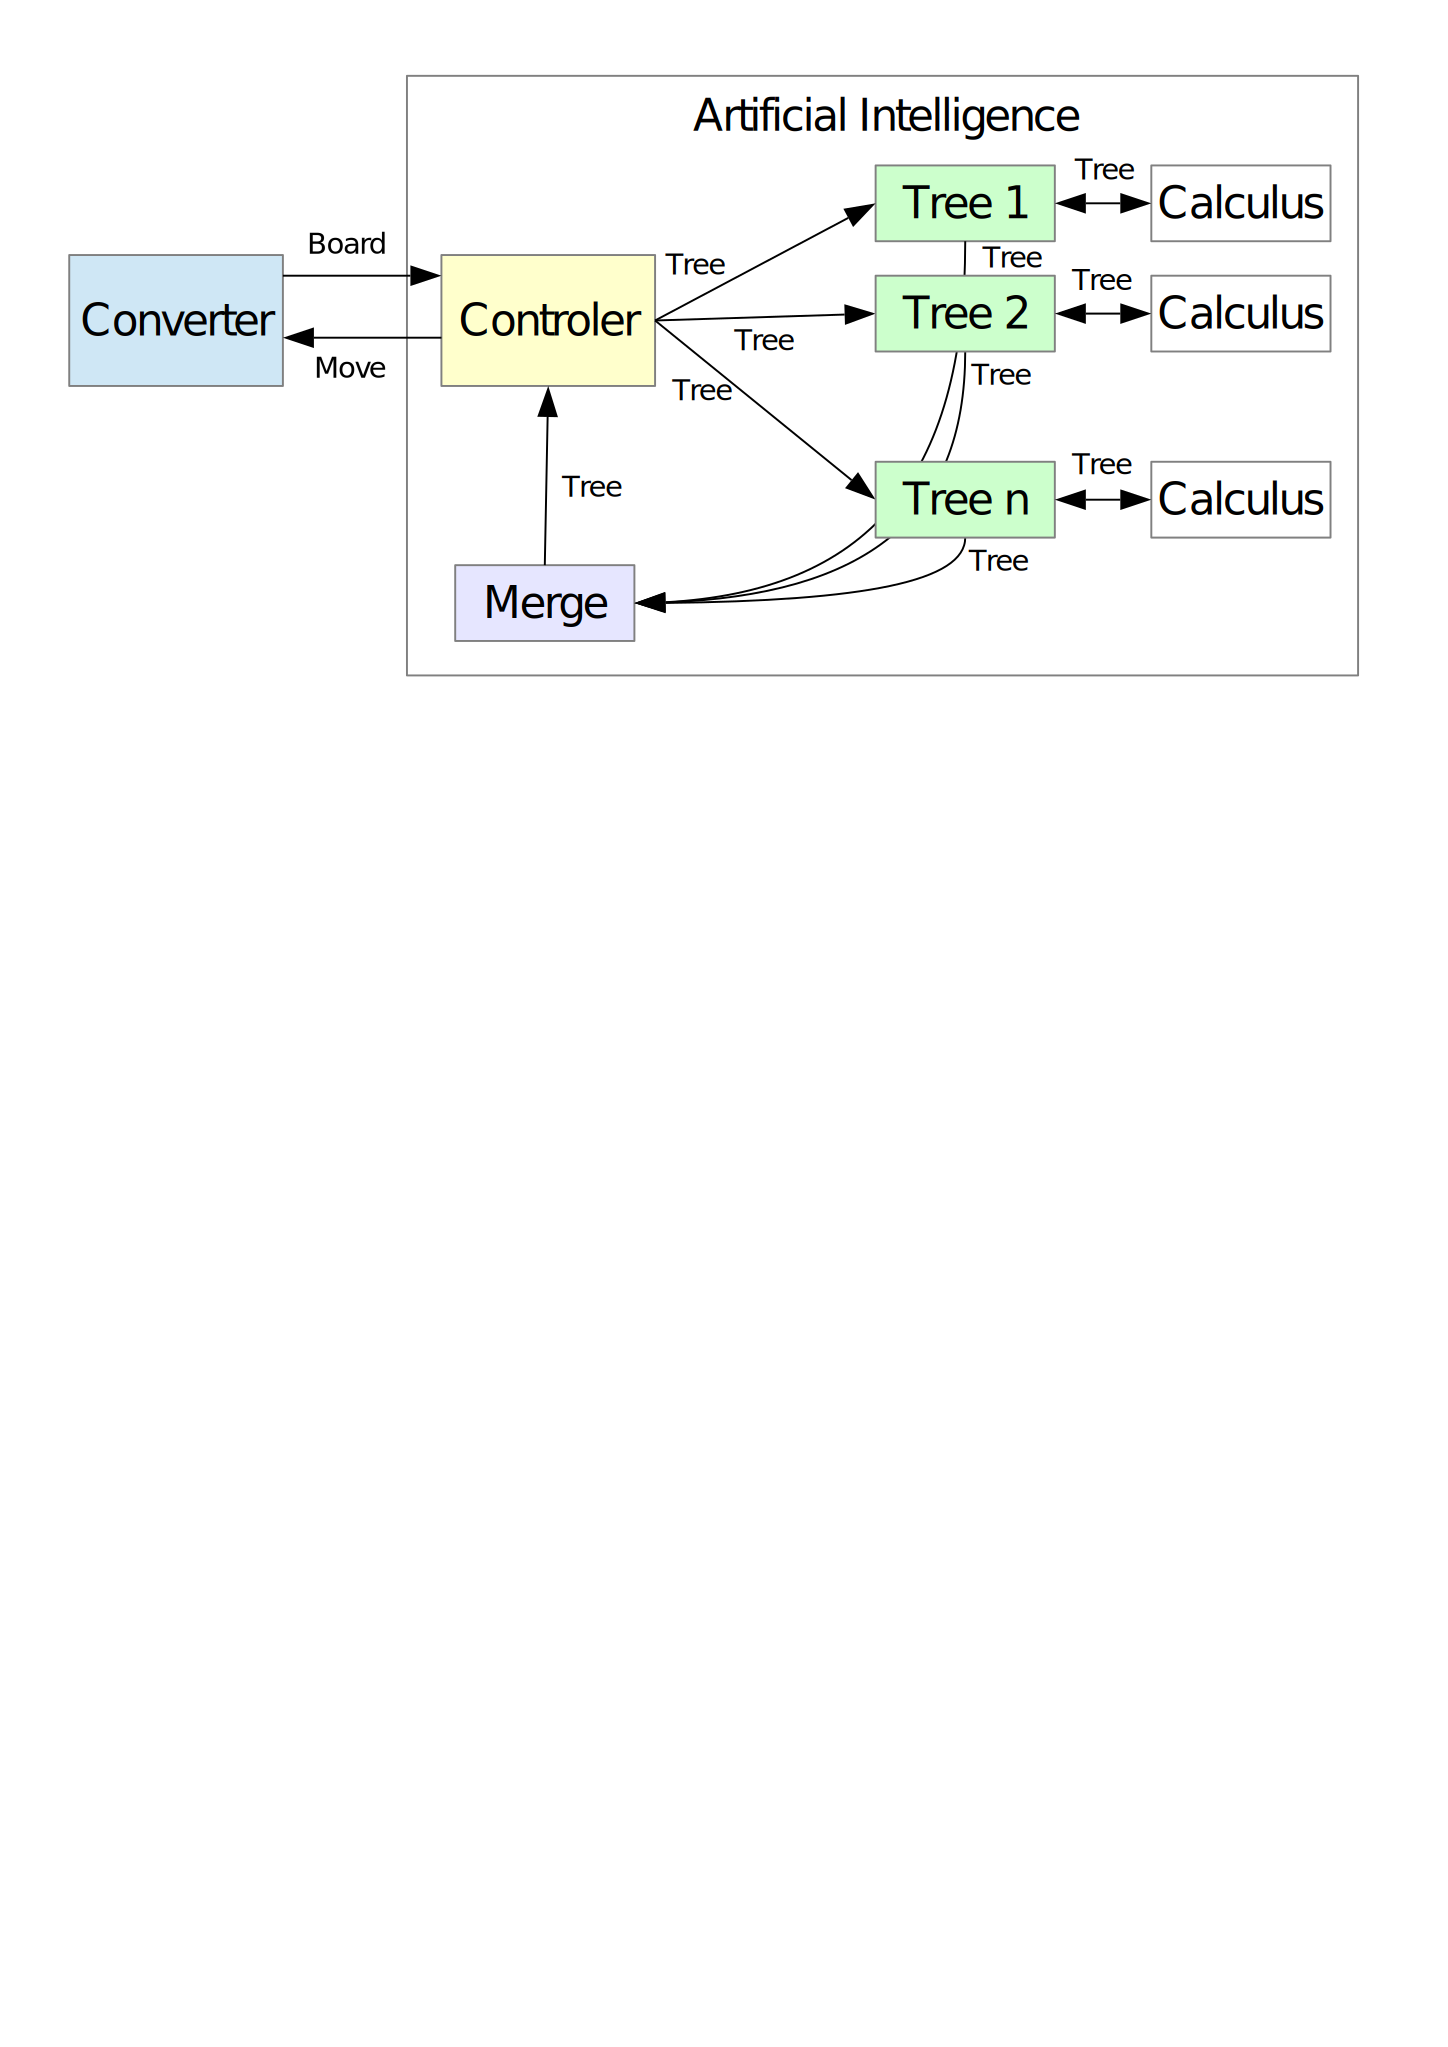
\includegraphics[width=0.80\textwidth]{2General_Architecture/2.3MCTS/AI.jpg}
	\caption{Artificial Intelligence}
	\label{fig:flow}
\end{figure}

The converter sends the state of the board to the controler, which creates trees of moves in different instances of the module. Each of these submodules computes simultaneously his tree, getting the possible moves thanks to a set of rules, represented here by the letter R. Furthermore, these submodules are able to evaluate each chosen move in a tree, comparing winrate and views.

Then, when the calculus is over, the submodules hands over the tree to the Merge module. When all instances of the module have done it, the Merge module merges the trees, gathering data in an only tree, that is sent to the controler.

Finally, the controler is able to decide what move to choose and it sent this move to the converter.


\newpage

\section{Software solutions}					\label{sec:softwareSolutions}
	\subsection{Shared memory Parallelism on CPU}	\label{sec:openmp}			To parallelize our algorithm on the CPU, we need to chose a framework. Four solutions have been found and compared :
\begin{itemize}
\item MPI
\item OpenMp
\item C++11 Threads (Boost)
\item Pthreads (C)
\end{itemize}

\subsubsection{MPI}
MPI is a library mainly dedicated to parallelization between differents machines, it could works on a single CPU but doesn't provide as many possibilites as its counterparts. Therefore we chose to not use it for that part of the implementation.

\subsubsection{Pthreads}
Pthreads is out of order because it is depreciated : it is a C library and the C++11 provides more efficiency and possibilities. The threads management is heavy to code and requires a good knowledge of how threads works precisely.

\subsubsection{OpenMP and C++11}
OpenMP and C++11 are the only remaining options. C++11 is a simplification of the Boost library inducing the later to be more complete. The following table sumurizes each libriraries pros and cons :
\begin{center}
\begin{tabular}{| l | l | l |}
\hline
\multicolumn{1}{| c}{OpenMP} &\multicolumn{1}{| c}{C++11 Threads} &\multicolumn{1}{| c |}{ Pthreads (C) } \\
\hline
+ Options & + Flexibility & + Flexibility \\
+ Portable & + Type-Safety & + Low-level \\
+ Languages & + Possibilities & + Compatibility \\
- Performances & - Fortran & - Efforts \\
- Memory & - Compiler & - Type-safety \\
- Unreliable & - Scalling & - Management  \\
\hline
\end{tabular}
\end{center}

Both libraries get similar performances\footnote{http://www.cs.colostate.edu/~cs675/OpenMPvsThreads.pdf}. However OpenMP is easier to use (precompilier declarations...) and keeps the code clean. C++11 allows a better thread management. Nevertheless it also can easily fall behind his counterpart in term of speed if some mistakes are made : a high price has to be paid.

Considering OpenMP safer to use and get similar results to C++11, we chosed OpenMP to parallelize our algorithm on CPU.
	\subsection{Shared memory Parallelism on GPU}	\label{sec:openacc}			\input{4Software_Solution/4.2OpenACC/OpenACC.tex}
	\subsection{Cluster Parallelism}			\label{sec:mpi}				Our last software need is about the cluster parallelization. As we have decided to use a Root Parallelization there will not be a lot of communication between different computers, we could choose between two solutions: the Sockets and MPI.
\begin{itemize}
\item A socket is used to communicate across a computer network. The socket is an end point of the communication flow. A socket is a low-level mechanism.
\item MPI is a standardized message-passing system. It allows us to communicate between computers which belong to a network by sending messages between them. 
\end{itemize}
\subsubsection{The chosen solution}

We decided to use MPI for many reasons.
\begin{itemize}
\item MPI is more high-level than the sockets. So, it will be simpler to implement in our software.
\item The community behind MPI is large so there wouldn't be any problem to fix the different bugs. Moreover, the MPI documentation is clearer than the sockets' one. 
\item The operation of MPI is based on the sockets so it is similar, though a little bit inferior, to the sockets, in term of performances.
\end{itemize}
In conclusion, MPI would be simpler to implement, more documented than the sockets while they both have almost similar performance.
	\subsection{Actor Model}				\label{sec:actorModel}			In parts \ref{sec:openmp} to \ref{sec:mpi}, three solutions allowing the parallelization of our algorithm have been presented. In this part, the actor model, another way to handle parallelization, will be introduced.

In this model, every machine, core and GPU is seen as an actor. These actors can send messages to each other, using adresses. When they receive one, they can:
\begin{itemize}
\item send messages to other actors
\item create new actors
\item adapt their behavior
\end{itemize}

These actions can be realized in parallel. Moreover, the message system is totally asynchronus which is adapted to the root parallelization we will use at first. However, it will not be as interesting for other parallelization methods. For the moment we have not yet found a framework implementing the actor model that we could use for our project, but we are still looking for one, as it would be a very efficient solution. 
\newpage

\section{Conclusion}						\label{sec:conclusion}			The software specifications have been decided : further to the AI, a user interface (\emph{UI}) will be developed.
It will include every version of the AI that will have shown satisfying results.
Therefore, this project will be composed of three parts : the UI, the AI and the game model that will handle the rules.

The AI will use the \emph{Monte Carle tree search} algorithm.
In order to make it more efficient, it will implement parallelization on threads and on multiple machines.
If the machines at our disposal dispose of GPUs, they will also be used.
Ultimately, the goal is to try and run our algorithm on \emph{Grid 5000}, a set of clusters of multi-core machines.
This parallelisation will be performed using OpenMP and OpenACC on every machine, and MPI between machines.
We will first use \emph{Root parallelization}, and then try other strategies if there's enough time to do so.

The next step will be about defining the details of the implementation, before starting developement.
\newpage

%uncomment to add bibliography
\bibliography{bibliography}
\bibliographystyle{plain}

\end{document}
